\documentclass[11pt,slovak,twosides,openany]{scrbook}
\usepackage{fontspec}
\setmainfont[Ligatures=TeX]{Latin Modern Roman}
\setsansfont[Ligatures=TeX]{Latin Modern Sans}
\setmonofont{Latin Modern Mono}
\usepackage[a5paper]{geometry}
\geometry{verbose,rmargin=2.3cm}
\usepackage{fancyhdr}
\pagestyle{fancy}
\setcounter{secnumdepth}{3}
\setcounter{tocdepth}{0}
\usepackage{color}
\usepackage{babel}
\usepackage{array}
\usepackage{verbatim}
\usepackage{longtable}
\usepackage{graphicx}
\usepackage[unicode=true,pdfusetitle,
 bookmarks=true,bookmarksnumbered=false,bookmarksopen=false,
 breaklinks=false,pdfborder={0 0 0},backref=false,colorlinks=true]
 {hyperref}

\makeatletter

%%%%%%%%%%%%%%%%%%%%%%%%%%%%%% LyX specific LaTeX commands.
%% Because html converters don't know tabularnewline
\providecommand{\tabularnewline}{\\}

%%%%%%%%%%%%%%%%%%%%%%%%%%%%%% User specified LaTeX commands.
%%% CONSTANTS
\newcommand{\nadpis}{Matfyzákov sprievodca galaxiou}
\newcommand{\akademickyRok}{2013/2014}

%%% PACKAGES
\usepackage{booktabs}% for much better looking tables
\usepackage{array}% for better arrays (eg matrices) in maths
\usepackage{paralist}% very flexible & customisable lists (eg. enumerate/itemize, etc.)

%%% HEADERS & FOOTERS
\usepackage{fancyhdr} % This should be set AFTER setting up the page geometry
\pagestyle{fancy} % options: empty , plain , fancy
\renewcommand*{\chapterpagestyle}{fancy}
%\renewcommand{\headrulewidth}{0pt} % customise the layout...
\fancyhf{}
\chead{}
\fancyfoot[LE,RO]{\thepage}
\fancyhead[LE,RO]{\nadpis}
\fancyhead[LO,RE]{\akademickyRok}

%%% ToC (table of contents) APPEARANCE
\usepackage[titles]{tocloft} % Alter the style of the Table of Contents
\renewcommand{\cftsecfont}{\rmfamily\mdseries\upshape}
\renewcommand{\cftsecpagefont}{\rmfamily\mdseries\upshape} % No bold!

% removing space above chapter
\renewcommand*{\chapterheadstartvskip}{\vspace*{0cm}}

% font sizes
\setkomafont{chapter}{\normalfont\bfseries\fontsize{13}{15.5}\selectfont\scshape}
\setkomafont{section}{\normalfont\fontsize{13}{15.5}\selectfont}
\setkomafont{subsection}{\normalfont\bfseries}

\usepackage{longtable}

\makeatother

\begin{document}
\title{\nadpis}
\date{\akademickyRok}


\subtitle{Praktické rady a informácie pre štúdium}


\author{Pripravil ŠKAS}


\publishers{
\begin{figure}
\centering{}
\includegraphics[width=0.6\textwidth]{images/fmfi_logo}
 \end{figure}
}


\lowertitleback{Pripravila:\\
Študentská komora Akademického senátu (ŠKAS)\\
Fakulta matematiky, fyziky a informatiky\\
Univerzita Komenského v Bratislave\\
\\
\href{http://skas.fmph.uniba.sk}{http://skas.fmph.uniba.sk}\\
\href{https://www.facebook.com/MatFyzJeIn}{https://www.facebook.com/MatFyzJeIn}\\
\href{mailto:skas@skas.fmph.uniba.sk}{skas@skas.fmph.uniba.sk}\\
\\
Autori:\\
Kristián Valentín, Zuzana Cocuľová, Matúš Balogh,\\
Róbert Kysel\\
\\
Vydanie pre akademický rok 2013/2014.\\
\\
Sadzba pomocou programu \LaTeX.\\*
Ďalšie použité programy: LyX, Inkscape, GIMP.}

\maketitle
\tableofcontents{}

%\mainmatter\cleardoublepage

\chapter{Úvod}

Milá matfyzáčka, milý matfyzák,

vitaj na svojej novej Alma mater, na Matfyze! Blahoželáme ti k~prijatiu
a želáme veľa šťastia v štúdiu na našej fakulte.

Všetci sme raz boli prváci a zápasili sme s problémami, aké môžu stretnúť
aj Teba. Cieľom tejto publikácie je pomôcť ti zorientovať sa v~škole,
poradiť čo ako funguje, na koho sa máš obrátiť, kde sa dobre najesť,
požičať skriptá a podobne.

Máme pre Teba aj rozšírenú elektronickú verziu, ktorú si môžeš stiahnuť
zo ŠKAS stránky%
\footnote{\href{http://skas.fmph.uniba.sk}{http://skas.fmph.uniba.sk}%
}, príp. pomocou QR kódu:

\begin{center}

\includegraphics[width=0.17\textwidth]{images/qr_code}
\par\end{center}

\section{Čo je ŠKAS?}

ŠKAS je skratka pre Študentskú komoru Akademického senátu FMFI UK
a my sme jej členovia. Sme študenti, ktorí sa rozhodli, že chcú vo
svojom voľnom čase pracovať na zlepšení celkovej kvality štúdia a
študentského života na fakulte. 

Členovia ŠKASu sú volení študentmi FMFI a reprezentujú ich v akademickom
senáte. Akademický senát FMFI UK je samosprávny zastupiteľský orgán,
ktorý rozhoduje na svojich zasadnutiach o dôležitých otázkach fungovania
fakulty. 

<%
# vymazem uvod (je uz v template)
remove_until = '\chapter{Štúdium}'
index = body.index(remove_until)# + remove_until.length
body = body[index..-1]

# vymazem sekcie pri mapach
body = body.sub('\section{Mapa Mlynskej doliny}\hypertarget{mapa-mlynskej-doliny}{}\label{mapa-mlynskej-doliny}', '')
body = body.sub('\section{Mapa Matfyzu}\hypertarget{mapa-matfyzu}{}\label{mapa-matfyzu}', '')

# upravim velkost obrazkov
body = body.sub('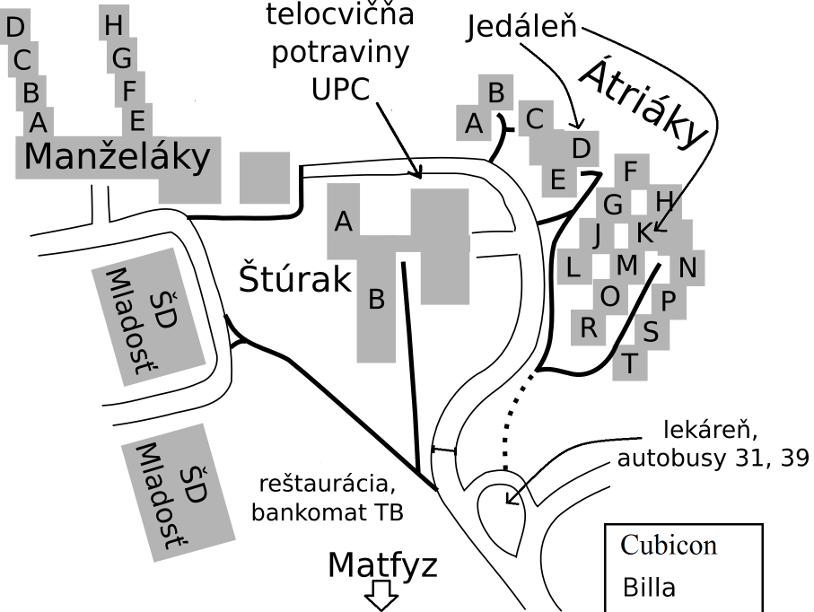
\includegraphics{images/mapa-horiz_w.png}', '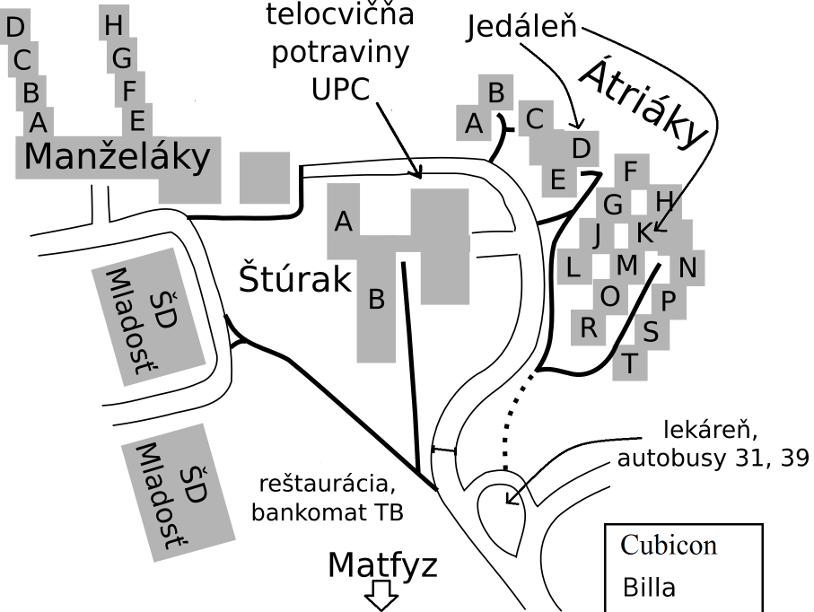
\includegraphics[width=1\textwidth]{images/mapa-horiz_w.png}')
body = body.sub('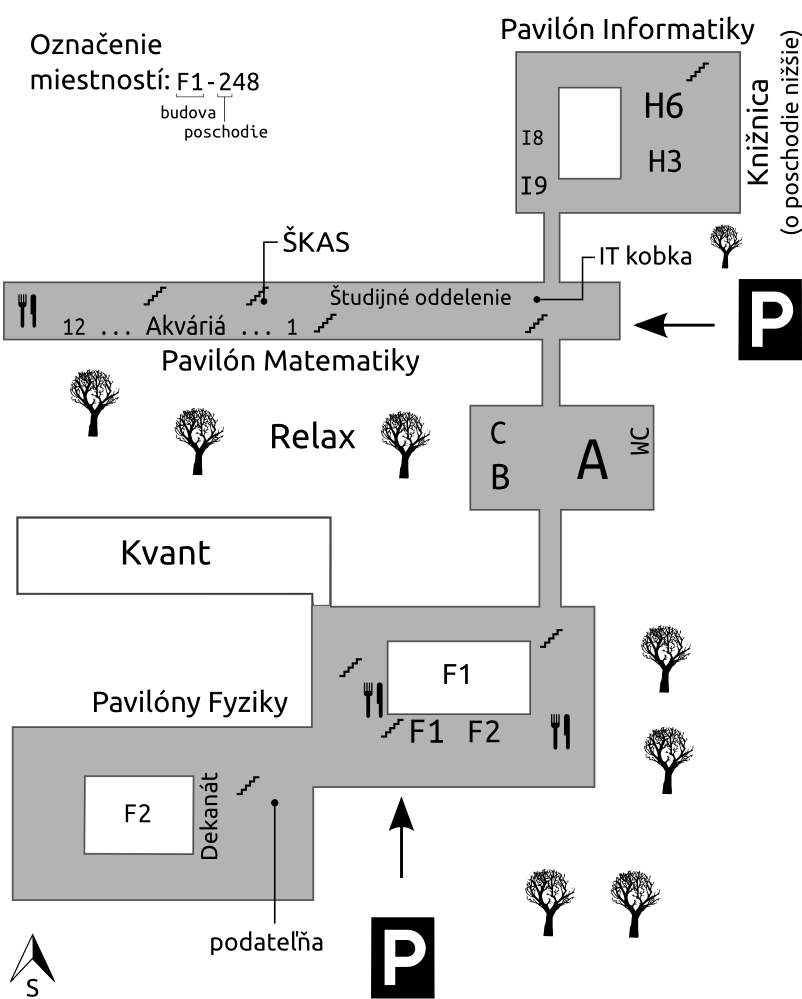
\includegraphics{images/plan_matfyzu.png}', '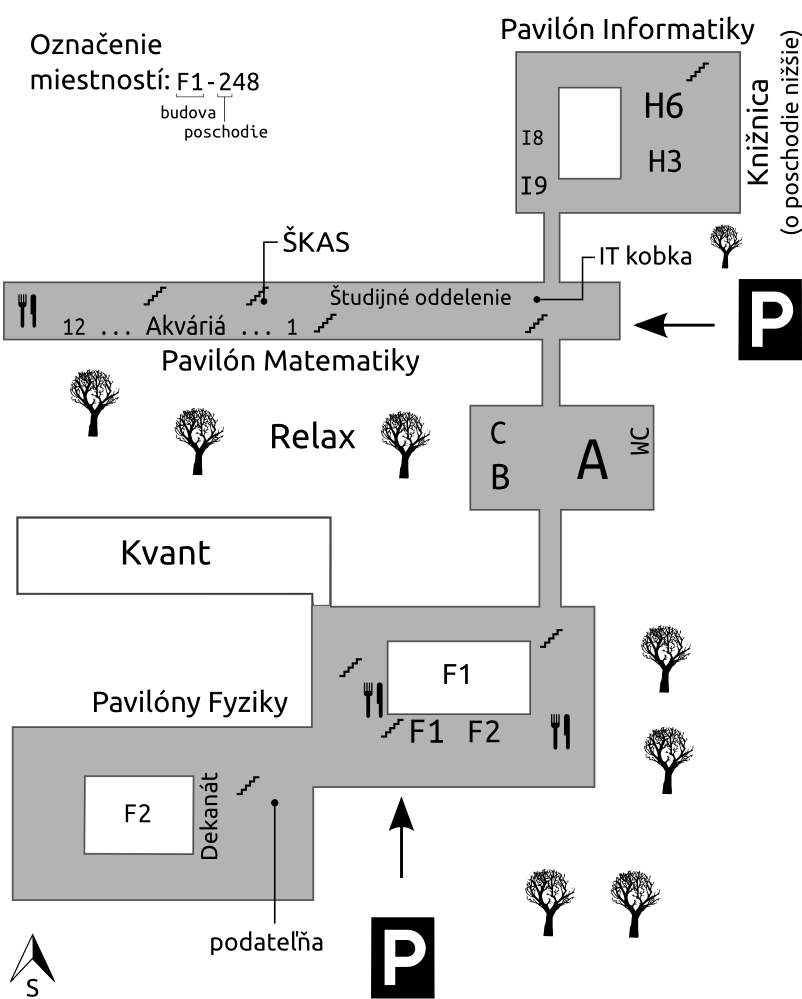
\includegraphics[width=1\textwidth]{images/plan_matfyzu.png}')
%>

<%= body %>

\end{document}
